%\documentclass[a4paper,11pt]{article}
\documentclass[journal]{IEEEtran}
\usepackage[pdftex]{graphicx}
\usepackage[pdftex, pdftitle={}, pdfauthor={}, pdfkeywords={},pdfstartview=FitB]{hyperref}
\usepackage{subfig}
\usepackage{booktabs}
\usepackage{tikz}
\usepackage[numbers]{natbib}
\bibliographystyle{IEEEtran}

\usepackage{soul}

\begin{document}
\title{Reproducing Social Networks from Anonymous Community Networks}

\author{Norbert~B\'atfai, 
M\'at\'e Smajda,
Szir\'aki Szabolcs,
Erika~B\'atfai%
\thanks{N. B\'atfai is with the Department of Information Technology, University of Debrecen,
H-4010 Debrecen PO Box 12, Hungary, e-mail: batfai.norbert@inf.unideb.hu.}
\thanks{M\'at\'e Smajda,
Szir\'aki Szabolcs,
Erika~B\'atfai
are with the University of Debrecen.}
}

\maketitle

\begin{abstract}
In this paper, we present an application, called YANonymous. It attempts to reproduce the global social network from its users' anonymous community networks. In parallel with this, we show results of a concrete experiment in which we try to develop a procedure to predict the behavior of the citizens in the Hungarian parliamentary election. The suggested prediction mechanism is entirely based on the social network reproduced  from the citizens' own anonymous community networks by the application YANonymous.
\end{abstract}

\begin{IEEEkeywords}
social networks, community networks, Hungarian parliamentary election
\end{IEEEkeywords}

\section{Introduction}
In our opinion it is possible to manufacture a social network from anonymous social nets. We can collect anonymous party preference information and then we can map a wider community network with the software which has been developed for this goal. The provided subgraphs are going into the YANonymous application and there the real social net will be outlined from the various anonymous networks with using the one-way, one-distance relations.

\subsection{Related Works}


\hl{Simulation and Modeling}

\hl{Repast Suite}

\cite{repast}

\hl{Axelrod culture model}

\cite{zuckbook}, \cite{axelrod0}, \cite{axelrod1}, \cite{axelrod2}

\hl{Swarm simulation toolkit}

\cite{swarm}


\subsection{The Development Methodology}
As main method we choiced the social-network analysis, because this method provides the rather tangible results to our program. 
Why doesn’t the sociometry? The interpersonal relationships are explored quantitative by the sociometrics. The sociometry is the method of the close groups primarily. Its profits might are illustrated by sociogram or by reciprocal matrix (Mérei p. 50-58.).

The pitfalls of the poll are divided to sampling and no sampling faults. In our case the sampling isn’t interpreted, because the purpose of research doesn’t replicate the various, which is occurred in the population (this is effective and valid in good case), instead of  real occurrence. Which is based on the goodness of social net might is generate.
So the compromise on sampling doesn’t need too and the limit of error no problem, as well as the various are likely to representative. 

The data collections was being run in our loose, personal social capital. Therefore we can define the companionship for networking, the type of relationship exactly. 
At issue what extent does the so created pattern cover the nation-wide pattern, which existence is based on no social capital.

We concocted our net very simply: margin of our net was marked out by ourselves with the nominalist approach. There wasn’t goal mapping of  the whole network of contacts, just an certain amount of real data were needed, which were no mirror and we didn’t conclude based on these to larger community reviews, however these gave basis of social net goodness’. That is we had a central ego-net  \cite{kurtosi}. The destiny of links and reciprocity of links are irrelevant too. 
The data collection through questionnaire proves to was most appropriate, because specified  number of connection was needed.

We used an application on the tablet to the collection.The asked person indicated party preferences of own social net points and their relations.  The data were storaged in the tablet without ID.
We needed the more local subgraphs to manufacture an real social network, to this end we looked for people with similar affiliations (e.g. place of residence, workplace, university).

\subsection{The Hungarian Parliamentary Election}

The Hungarian voting right is equivalent and general. Every 18-years old and more Hungarian citizen with Hungarian address are entitled to vote. The election own is secret and no compulsory.

People have got 199 representatives (106 personal and 93 listed) into the parliament since 2012 via one-round, two-votes election, when the citizen can vote 1 personal representative and 1 listed representative. Those parties may posit nationwide partylist, whose have candidate at least in the 9 counties and in the capital constituencies, independently. 

We had to wait the finals partylist of Hungarian parlamentary election, 2014  to my  data collenction. We could vote 18 partylists, which based on the decision of the National Election Commission, on this election.


\section{Reproducing Social Networks from Anonymous Community Networks}

\subsection{The YANonymous Application}

The basic relationship types are listed in Table \ref{fig:table:rels}.

yano $\to$ grandmother $=$ yano $\to$ mother $\to$ mother

yano $\to$ brother $=$ yano $\to$ mother $\to$ son or yano $\to$ father $\to$ son  
      

\begin{table}[!h]
  \centering
  \subfloat[][]{\begin{tabular}{l}
    \toprule
    $yano \to mother$ \\
    \midrule
    $yano \to wife$ \\
    \midrule
    $yano \to daughter$ \\
    \midrule
    $yano \to girlfriend$ \\
        \midrule
    $yano \to friend$ \\
      \midrule
    $yano \to neighbour$ \\
      \midrule
    $yano \to classmate$ \\
     \midrule
    $yano \to colleague$ \\
    \bottomrule
  \end{tabular}}
  \qquad
  \subfloat[][]{\begin{tabular}{l}
    \toprule
    $yano \to father$ \\
    \midrule
    $yano \to husband$ \\
    \midrule
    $yano \to son$\\
    \midrule
    $yano \to boyfriend$ \\
      \midrule
    $yano \to acquaintance$ \\
      \midrule
    $yano \to housemate$ \\
    \midrule
    $yano \to teammate$ \\
    \midrule
    $yano \to ex$ \\
    \bottomrule
  \end{tabular}}
  \caption{The basic relationship types.}
  \label{fig:table:rels}
\end{table}

\begin{figure}[!h]
\begin{center}
\small
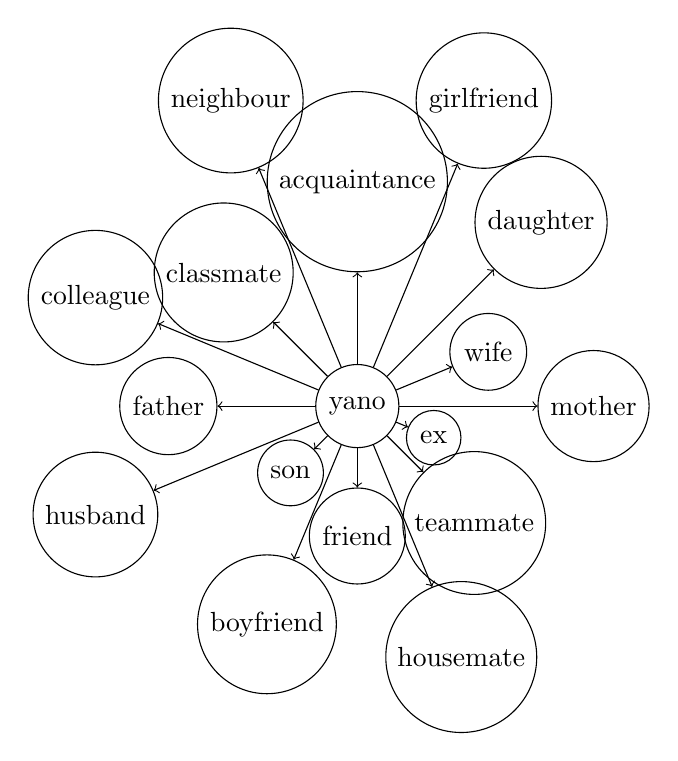
\begin{tikzpicture}[scale=3]
\tikzstyle{every node}=[draw,shape=circle];
\draw (0:0cm) node       (y0) {yano};
\draw (0:1cm) node       (y1) {mother};
\draw (22.5:0.6cm) node  (y2) {wife};
\draw (45:1.1cm) node      (y3) {daughter};
\draw (67.5:1.4cm) node  (y4) {girlfriend};
\draw (90:0.95cm) node      (y5) {acquaintance};
\draw (112.5:1.4cm) node (y6) {neighbour};
\draw (135:0.8cm) node     (y7) {classmate};
\draw (157.5:1.2cm) node (y8) {colleague};
\draw (180:0.8cm) node     (y9) {father};
\draw (202.5:1.2cm) node (y10) {husband};
\draw (225:0.4cm) node     (y11) {son};
\draw (247.5:1cm) node   (y12) {boyfriend};
\draw (270:0.55cm) node     (y13) {friend};
\draw (292.5:1.15cm) node   (y14) {housemate};
\draw (315:0.7cm) node     (y15) {teammate};
\draw (337.5:0.35cm) node (y16) {ex};

\tikzset{every node/.style={fill=white}} 
\draw (y0) edge [->] (y1);
\draw (y0) edge [->] (y2);
\draw (y0) edge [->] (y3);
\draw (y0) edge [->] (y4);
\draw (y0) edge [->] (y5);
\draw (y0) edge [->] (y6);
\draw (y0) edge [->] (y7);
\draw (y0) edge [->] (y8);
\draw (y0) edge [->] (y9);
\draw (y0) edge [->] (y10);
\draw (y0) edge [->] (y11);
\draw (y0) edge [->] (y12);
\draw (y0) edge [->] (y13);
\draw (y0) edge [->] (y14);
\draw (y0) edge [->] (y15);
\draw (y0) edge [->] (y16);
 \end{tikzpicture}
 \caption{A graph representation of thebasic relationship types.}
  \label{fig:img:grapgrep}
  \end{center}
\end{figure}


\subsubsection{YANonymous Construct}

\subsubsection{YANonymous Puzzle}

\subsection{Experimental Results}

\section{Conclusion}

\section*{Acknowledgment}

The authors would like to thanks 
the members of the Google-group ``yanonymous@googlegroups.com'' and especially   
the students of the BSc courses of ``Java casestudies'' and "Programming"
in the winter semester of 2013/2014 at the University of Debrecen 
for monitoring and participation in development of the YANonymous.

The publication was supported by the T\'AMOP-4.2.2.C-11/1/KONV-2012-0001 project. The project has been supported by the European Union, co-financed by the European Social Fund.


\begin{IEEEbiography}[{
\includegraphics[width=1in,height=1.25in,clip,keepaspectratio]{images/bn}}]{Norbert~B\'atfai}
is working as an assistant professor in Faculty of Informatics at the University of Debrecen, Hungary. He received his M.Sc. (summa cum laude) in Computer Science at 1998 from the Kossuth Lajos University (KLTE), Debrecen, Hungary. In 1999, he won the first prize in the Java Programming Contest organized by Hungarian Java Alliance: Sun, IBM, Oracle, Novell and IQSoft. In 2004, his company won the first prize in the Hungarian Mobile Java Developer Contest organized by Sun Hungary and Nokia Hungary. In 2008, the Hungarian Chief Information Officers' Association has selected him as an IT trainer of the year. He received the Ph.D degree in 2011. He won the Poll\'ak-Vir\'ag award from Scientific Association for Infocommunications Hungary in 2012.
\end{IEEEbiography}


\bibliography{yanonymous}

\end{document}
